\subsection{Wasserstein 距离}\label{sec:1.2}

Kantorovich 问题 \eqref{eq:KOT} 对许多不同的成本函数都有意义，而每种情形都有不同的解释. 例如，一个自然的例子是取平凡度量 $c(x,y)=\mathbbm{1}_{x\ne y}$. 此时 \eqref{eq:KOT} 给出
$$
\inf_{\gamma\in\Gamma_{\mu,\nu}}\gamma(X\ne Y),
$$
这是全变差距离（total variation distance）的一个熟知表述，见\autoref{exer:9}. 然而，注意平凡距离 $\mathbbm{1}_{x\ne y}$ 与 $\mathbb R^d$ 的几何无关. 特别地，它只区分 $x$ 与 $y$ 是否不同，而不说明两者相距多远. 全变差也表现出这一局限. 事实上，若 $\mu=\delta_x$、$\nu=\delta_y$，则只要 $x\ne y$，\eqref{eq:KOT} 的目标值就等于 $1$.

要从 Kantorovich 问题得到一个具有几何意义的量，就必须选择能反映 $x$ 与 $y$ 之间实际距离的成本. 这个想法导出了 Wasserstein 距离. 对任意 $p\ge1$，用 $\mathcal P_p(\mathbb R^d)$ 表示配备欧氏范数 $\lVert\cdot\rVert$ 的 $\mathbb R^d$ 上所有具有有限 $p$ 阶矩的概率测度组成的集合：
$$
\mu\in\mathcal P_p(\mathbb R^d)
\quad\Longleftrightarrow\quad
\int\lVert x\rVert^p\,\mu(dx)<\infty.
$$
两个概率测度 $\mu,\nu\in\mathcal P_p(\mathbb R^d)$ 之间的 $p$-Wasserstein 距离定义为
$$
W_p(\mu,\nu)=\inf_{\gamma\in\Gamma_{\mu,\nu}}
\left(\int\lVert x-y\rVert^p\,\gamma(dx,dy)\right)^{1/p},
$$
其中回顾一下，$\Gamma_{\mu,\nu}$ 是 $\mu$ 与 $\nu$ 的耦合集合.

首先证明，上述下确界实际上能够达到. 为此，定义
$$
I(\gamma):=\int\lVert x-y\rVert^p\,\gamma(dx,dy),
$$
注意根据定义，存在 $\Gamma_{\mu,\nu}$ 中的序列 $(\gamma_n)_n$，使 $I(\gamma_n)\to W_p^p(\mu,\nu)$. 由于 $\Gamma_{\mu,\nu}$ 是紧的（\autoref{prop:1.1}），$(\gamma_n)_n$ 有一个子序列收敛到某个 $\bar\gamma\in\Gamma_{\mu,\nu}$. 根据定义，$W_p(\mu,\nu)\le I(\bar\gamma)$. 由于 $(x,y)\mapsto\lVert x-y\rVert^p$ 无界，$I$ 并不连续，但它是下半连续的，因此 $I(\bar\gamma)\le\liminf_{n\to\infty}I(\gamma_n)=W_p^p(\mu,\nu)$（portmanteau 定理的第三条，\autoref{thm:B.4}）. 从而 $I(\bar\gamma)=W_p^p(\mu,\nu)$. 注意，这个证明中关于成本函数所用的唯一性质就是下半连续性，因此该论证很容易推广到更一般的成本.

由此，可以采用如下 Wasserstein 距离的定义. 注意，这些距离实际上应该称为 Kantorovich--Rubinstein 距离，不过我们仍沿用当下的“Wasserstein 化”潮流.

\begin{definition}\label{def:1.2}\index{Wasserstein distance@Wasserstein距离（Wasserstein distance）|hyperpage}
两个概率测度 $\mu,\nu\in\mathcal P_p(\mathbb R^d)$ 之间的 $p$-Wasserstein 距离定义为
$$
W_p(\mu,\nu)=\min_{\gamma\in\Gamma_{\mu,\nu}}
\left(\int\lVert x-y\rVert^p\,\gamma(dx,dy)\right)^{1/p}.
$$
\end{definition}

\Needspace{8\baselineskip}
\begin{proposition}\label{prop:1.3}
$p$-Wasserstein 距离在 $\mathcal P_p(\mathbb R^d)$ 上定义了一个度量，即对任意 $\mu,\nu\in\mathcal P_p(\mathbb R^d)$：
\begin{enumerate}
\item\label{item:1.3.1} $W_p(\mu,\nu)\ge0$.
\item\label{item:1.3.2} $W_p(\mu,\nu)=W_p(\nu,\mu)$.
\item\label{item:1.3.3} $W_p(\mu,\nu)=0$ 当且仅当 $\mu=\nu$.
\item\label{item:1.3.4} 对任意 $\rho\in\mathcal P_p(\mathbb R^d)$，$W_p(\mu,\nu)\le W_p(\mu,\rho)+W_p(\rho,\nu)$.
\end{enumerate}
\end{proposition}
\begin{proof}
首先注意，\hyperref[item:1.3.1]{第 1 条}和\hyperref[item:1.3.2]{第 2 条}显然成立.

现在证明\hyperref[item:1.3.3]{第 3 条}. 若 $\mu=\nu$，则测度 $\gamma(dx,dy)=\mu(dx)\delta_x(dy)$ 是有效耦合，即 $\gamma\in\Gamma_{\mu,\nu}$. 具体地，$\gamma$ 是 $X\sim\mu$ 时 $(X,X)$ 的分布. 因此
$$
0\le W_p^p(\mu,\mu)\le\int\lVert x-y\rVert^p\,\gamma(dx,dy)
=\int\lVert x-x\rVert^p\,\mu(dx)=0.
$$
为证明\hyperref[item:1.3.3]{第 3 条}的反方向，注意若 $W_p(\mu,\nu)=0$，则存在 $\bar\gamma\in\Gamma_{\mu,\nu}$，使 $(X,Y)\sim\bar\gamma$ 且 $X=Y$ 几乎必然成立；特别地，它们必然同分布，即 $\mu=\nu$.

为完成证明，检验\hyperref[item:1.3.4]{第 4 条}的三角不等式. 为此使用粘合引理（gluing lemma，\autoref{lem:B.5}），它保证存在 $X,Y,Z$，满足 $X\sim\mu$、$Y\sim\nu$、$Z\sim\rho$，并且 $(X,Z)$ 与 $(Z,Y)$ 都是最优耦合. 于是
$$
\begin{aligned}
W_p(\mu,\nu)
&\le\bigl(\mathbb E\lVert X-Y\rVert^p\bigr)^{1/p}\\
&=\bigl(\mathbb E\lVert X-Z+Z-Y\rVert^p\bigr)^{1/p}\\
&\le\bigl(\mathbb E\lVert X-Z\rVert^p\bigr)^{1/p}
+\bigl(\mathbb E\lVert Z-Y\rVert^p\bigr)^{1/p}\\
&=W_p(\mu,\rho)+W_p(\rho,\nu),
\end{aligned}
$$
其中第一行使用了耦合 $(X,Y)$ 的次优性，第三行使用了 $L^p$ 范数的三角不等式，最后一行使用了耦合 $(X,Z)$ 与 $(Z,Y)$ 的最优性.
\end{proof}

\begin{example}[简单情形下的 Wasserstein 距离]\label{ex:1.4}\leavevmode
\begin{enumerate}
\item 固定 $x,y\in\mathbb R^d$，则
$$
W_p(\delta_x,\delta_y)=\lVert x-y\rVert.
$$
因此，$(\mathbb R^d,\lVert\cdot\rVert)$ 通过 $x\mapsto\delta_x$ 等距嵌入 $(\mathcal P_p(\mathbb R^d),W_p)$.
\item 固定 $x,y\in\mathbb R^d$ 及 $0\le\lambda,\tau\le1$，则
$$
W_p\bigl(\lambda\delta_x+(1-\lambda)\delta_y,\tau\delta_x+(1-\tau)\delta_y\bigr)
=|\lambda-\tau|^{1/p}\lVert x-y\rVert.
$$
\end{enumerate}
\end{example}

注意，由 $L^p$ 范数的序关系可知，只要 $p\le q$，就有 $W_p(\mu,\nu)\le W_q(\mu,\nu)$. 特别地，Wasserstein 距离中最小的是 $W_1$.

Wasserstein 距离在随机变量上诱导了一种有用的拓扑：它们使紧空间上的弱收敛度量化；相关背景见\autoref{sec:B}. 更具体地，序列 $(\mu_n)_n$ 满足 $W_p(\mu_n,\mu)\to0$，当且仅当它弱收敛于 $\mu$（记为 $\mu_n\rightsquigarrow\mu$），并且 $p$ 阶矩收敛，即 $\int\lVert\cdot\rVert^p\,d\mu_n\to\int\lVert\cdot\rVert^p\,d\mu$. 这种“度量化”性质可以在最优传输的所有主要教材中找到，也常被用来论证使用 Wasserstein 距离而不是其他距离的合理性. 然而，这几乎算不上一个能将它与其他距离区分开的特征：许多其他距离，例如 L\'evy--Prokhorov 距离、Fortet--Mourier 距离等，也具有这一性质，见\cite[第 6 章]{ref317}. 实际上，这个广为人知的结果并没有充分揭示对于某个 $\varepsilon$，$W_p(\mu,\nu)\le\varepsilon$ 所具有的定量含义.

例如，下面的命题说明，如果两个尾部足够轻的随机变量在任意 $p>1$ 的 $p$-Wasserstein 距离下接近，那么它们的所有矩也一定接近. 我们通过考虑次指数随机变量（sub-exponential random variable），来形式化尾部轻这一假设；这里指满足下式的随机变量 $Z$：
\begin{equation}\label{eq:1.4}
\mathbb E e^{|Z|}\le2.
\end{equation}
对于这样的随机变量，有如下界.

\begin{proposition}\label{prop:1.5}
设 $X\sim\mu$ 和 $Y\sim\nu$ 是两个次指数随机变量. 则对于任意 $p>1$，存在常数 $C_p>0$，使任意整数 $\ell\ge1$ 都满足
$$
\bigl|\mathbb E|X|^\ell-\mathbb E|Y|^\ell\bigr|
\le(C_p\ell)^\ell W_p(\mu,\nu).
$$
\end{proposition}
\begin{proof}
由函数 $x\mapsto|x|^\ell$（$\ell\ge1$）的凸性，
$$
|X|^\ell-|Y|^\ell
\le\ell|X-Y|\bigl(|X|^{\ell-1}\vee|Y|^{\ell-1}\bigr).
$$
对两边取期望，并应用 H\"older 不等式，得到对任意耦合 $(X,Y)$，
$$
\begin{aligned}
\bigl|\mathbb E|X|^\ell-\mathbb E|Y|^\ell\bigr|
&\le\ell\bigl(\mathbb E|X-Y|^p\bigr)^{1/p}
\bigl(\mathbb E(|X|^{\ell-1}\vee|Y|^{\ell-1})^q\bigr)^{1/q},\\
&\hspace{5em}\frac1p+\frac1q=1.
\end{aligned}
$$
取 $X$ 与 $Y$ 的最优耦合，得到
$$
\bigl|\mathbb E|X|^\ell-\mathbb E|Y|^\ell\bigr|
\le\ell W_p(\mu,\nu)
\bigl(\mathbb E(|X|^{\ell-1}\vee|Y|^{\ell-1})^q\bigr)^{1/q}.
$$
最后，回顾次指数随机变量的一个标准性质\cite{ref314}：若 $Z$ 是次指数的，则对所有 $k\ge1$，$\bigl(\mathbb E[|Z|^k]\bigr)^{1/k}\le k$. 因此
$$
\bigl(\mathbb E(|X|^{\ell-1}\vee|Y|^{\ell-1})^q\bigr)^{\frac1{(\ell-1)q}}
\le2(\ell-1)q\le2\frac{\ell p}{p-1}.
$$
\end{proof}

上述结果令人鼓舞：若得到两个测度之间 Wasserstein 距离的界，就能得到它们的矩之间距离的定量界. 不过，相较于其他常用距离或散度，例如全变差或 Kullback--Leibler 散度，Wasserstein 距离也可能往往相当大；关于这些距离的列表、彼此比较及其与统计问题的关系，见\cite[第 2 章]{ref302}.

然而，Wasserstein 距离通常可以由其他常用距离控制. 例如，下面的结果表明，在有界区域上，Wasserstein 距离受全变差距离控制（背景见\autoref{exer:9}）. 此外，它的证明首次展示了如何给出 Wasserstein 距离的界：只需构造一个（次优的）耦合 $\gamma$，使 $\mathbb E_\gamma\lVert X-Y\rVert^p$ 得到适当控制即可.

\begin{theorem}\label{thm:1.6}
设 $\mu,\nu\in\mathcal P_p(\mathbb R^d)$ 是两个分布，其密度分别为 $f$ 和 $g$. 则对任意 $p\ge1$，
$$
W_p^p(\mu,\nu)\le2^{p-1}\inf_{x_0\in\mathbb R^d}
\int\lVert x-x_0\rVert^p|f(x)-g(x)|\,dx.
$$
特别地，若 $\mu$ 和 $\nu$ 的支撑都包含在同一个直径为 $D$ 的球内，则
$$
W_p^p(\mu,\nu)\le D^p d_{\mathrm{TV}}(\mu,\nu),
$$
其中 $d_{\mathrm{TV}}(\mu,\nu)$ 是 $\mu$ 与 $\nu$ 之间的全变差距离，定义为
$$
d_{\mathrm{TV}}(\mu,\nu)=\frac12\int|f(x)-g(x)|\,dx.
$$
\end{theorem}
\begin{proof}
假设 $\mu\ne\nu$，否则结论显然成立. 正如定理陈述前所提到的，我们将构造 $\mu$ 与 $\nu$ 的一个显式耦合. 为此，考虑三个正函数 $(f-g)_+$、$(f-g)_-$ 与 $f\wedge g$（参见\autoref{fig:1.3}），并注意
$$
\int\bigl((f-g)_+-(f-g)_-\bigr)=\int f-\int g=1-1=0,
$$
\begin{figure}[htbp]
\centering
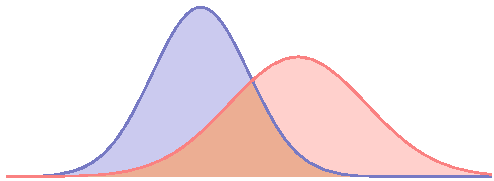
\includegraphics[width=\linewidth]{assets/chapter1/fig1-3.pdf}
\caption{积分 $\int(f-g)_+$、$\int(f-g)_-$ 与 $\int f\wedge g$ 分别对应蓝色、红色与橙色区域.}\label{fig:1.3}
\end{figure}

因此
$$
\int(f-g)_+=\int(f-g)_-=:t>0,
$$
并且
$$
\int f\wedge g
=\frac12\left(\int f+\int g-\int(f-g)_+-\int(f-g)_-\right)=1-t.
$$

接着，将这些函数归一化，得到三个密度
$$
h_+=\frac1t(f-g)_+,\qquad h_-=\frac1t(f-g)_-,\qquad
h_\wedge=\frac1{1-t}f\wedge g.
$$
可以将 $f$ 与 $g$ 重新写成上述密度的混合：
$$
f=th_++(1-t)h_\wedge,\qquad g=th_-+(1-t)h_\wedge.
$$
再令 $Z_+$、$Z_-$、$Z_\wedge$ 是三个相互独立的随机变量，其密度分别为 $h_+$、$h_-$、$h_\wedge$；令 $B$ 是参数为 $t\in(0,1]$ 的 Bernoulli 随机变量，且与 $Z_+$、$Z_-$、$Z_\wedge$ 独立.

现在可以定义 $\mu$ 与 $\nu$ 的耦合了. 为此，令随机变量对 $(X,Y)$ 满足
$$
\begin{aligned}
X&=BZ_++(1-B)Z_\wedge,\\
Y&=BZ_-+(1-B)Z_\wedge,
\end{aligned}
$$
注意 $(X,Y)$ 的分布 $\gamma$ 确实是 $\mu$ 与 $\nu$ 的有效耦合. 结合这一事实与不等式 $\lVert x-y\rVert^p\le2^{p-1}\bigl(\lVert x-x_0\rVert^p+\lVert y-x_0\rVert^p\bigr)$，得到
$$
\begin{aligned}
W_p^p(\mu,\nu)
&\le\mathbb E_\gamma\lVert X-Y\rVert^p\\
&=\mathbb P(B=0)\cdot0
+\mathbb P(B=1)\int\lVert x-y\rVert^p h_+(x)h_-(y)\,dx\,dy\\
&\le t2^{p-1}\left(\int\lVert x-x_0\rVert^p h_+(x)\,dx
+\int\lVert y-x_0\rVert^p h_-(y)\,dy\right)\\
&=t2^{p-1}\left(\int\lVert x-x_0\rVert^p\bigl(h_+(x)+h_-(x)\bigr)\,dx\right)\\
&=2^{p-1}\left(\int\lVert x-x_0\rVert^p\bigl((f-g)_+(x)+(f-g)_-(x)\bigr)\,dx\right)\\
&=2^{p-1}\left(\int\lVert x-x_0\rVert^p|f(x)-g(x)|\,dx\right).
\end{aligned}
$$
再对右端关于 $x_0$ 取最小值，即得结论. 第二个结论只需取 $x_0$ 为上述球的球心，便容易得到.
\end{proof}

$\mu$ 和 $\nu$ 绝对连续的假设是多余的；只要直接操作测度而不是密度，完全相同的证明仍然适用，只是记号会稍显晦涩；见\cite[定理 6.15]{ref317}.
